
\begin{figure}
    \centering
    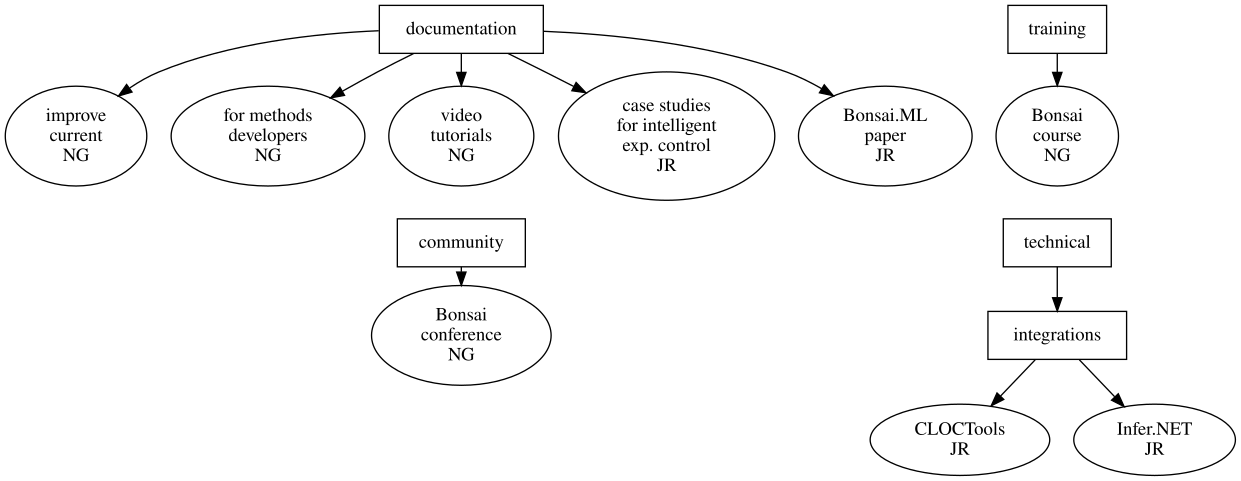
\includegraphics[width=6in]{activitiesGraphs/activities_larger.png}
    \caption{Proposed activities. See text for details.}
\end{figure}

\subsection*{Documentation}

Good documentation is essential for software uptake.
%
Bonsai.ML already contains substantial
\href{https://bonsai-rx.org/machinelearning/index.html}{documentation} for all
distributed packages. This documentation includes Bonsai working examples that users
can copy and paste them in their Bonsai local runtime and execute them. We will
extend this documentation by:

\begin{description}

    \item[providing more examples] on the application of the
        already integrated ML methods to new types of behavioural and
        neural data.

    \item[including video tutorials] on the use of the Bonsai.ML
        package.

    \item[adding documentation for methods developers] as the current one is
        targeted to Bonsai.ML users.

    \item[creating case studies] for intelligent experimental control in Bonsai,
        similar to the case studies for neural data analysis in
        Python\footnote[4]{\url{https://mark-kramer.github.io/Case-Studies-Python/intro.html}},
        or those for model based machine
        learning\footnote[5]{\url{https://mbmlbook.com/index.html}}, by our Microsoft
        collaborators.
        The aim of these case studies is to provide ML training to
        Bonsai users.

    \item[publishing a first Bonsai.ML paper] describing its functionality, as
        companion papers substantially increases the adoption of software
        packages \citep{lopesEtAl15,guilbeaultEtAl21}.

\end{description}

\subsection*{Training}

Since 2017, NeuroGEARS Ltd (the non-profit organisation that is the main
contributor to the development of Bonsai) has organised at least two Bonsai
course per year at different universities, and some of them can be viewed
online\footnote[5]{\url{https://bonsai-rx.org/learn/}}. We will organise a new
Bonsai course with a module on Bonsai.ML.

\subsection*{Community}

Adding state-of-the-art ML methods and comprehensive documentation is critical.
However, from our previous experience with Bonsai, adoption will be low if we
do not demonstrate the impact of Bonsai.ML methods for solving important
neuroscience problems.
%
For this, we need to work closely with experimental neuroscientists to help
them solve relevant problems in intelligent experimental control.

We will collaborate with experimental neuroscientists at the Sainsbury Wellcome
Centre (SWC; e.g., Prof.~Athena Akrami), at the Institute for Behavioral
Neuroscience (IBN) of University College London (Prof.~Aman Saleem), and at the
Allen Institute for Neural Dynamics (AIND; Dr.~Josh Siegle), on the integration
of machine learning functionality that we have already developed into their
experiments.
%
All these scientists are our close collaborators. Please refer to their letters
of support.

\subsection*{Integrations}

\subsubsection*{Probabilistic programming software: Infer.NET}

Most of the probabilistic models currently integrated into Bonsai are
implemented in Python. These serve as excellent demonstrations of how Python
applications can connect to the Bonsai ecosystem, and they are central to our
aim of attracting Python developers to contribute to Bonsai.ML.

However, Python implementations are substantially slower than equivalent C\#
code. For demanding real-time applications, C\# implementations are preferable,
especially when expressed in a probabilistic programming language (PPL).

The existing Python and C\# implementations of probabilistic models (e.g.,
linear dynamical systems, hidden Markov models, Bayesian linear regression —
see
\href{https://bonsai-rx.org/machinelearning/examples/README.html}{examples})
are relatively complex and heterogeneous, making them harder to maintain. In
contrast, implementations in a C\# PPL would be faster, simpler, and more
homogeneous, reducing errors and improving maintainability.

Fortunately, C\# has an excellent PPL:
\href{https://dotnet.github.io/infer/}{Infer.NET}, developed at Microsoft
Research Cambridge since 2004, used in
\href{https://dotnet.github.io/infer/papers.html}{hundreds of papers}, and
\href{https://www.microsoft.com/en-us/research/blog/the-microsoft-infer-net-machine-learning-framework-goes-open-source/}{open-sourced
in 2018}.  Infer.NET uses deterministic approximate inference, enabling fast
and scalable solutions. For example, it has powered systems that extract
knowledge from billions of web pages (petabyte-scale
data\footnote[7]{\url{https://www.microsoft.com/en-us/research/blog/the-microsoft-infer-net-machine-learning-framework-goes-open-source/}})
— the kind of scalability critical for real-time inference in Bonsai.

Message passing is a natural connection point between Bonsai and Infer.NET.
Infer.NET uses message passing for approximate inference, while Bonsai relies
on message passing for reactive computations. Exposing Infer.NET’s message
passing algorithms as Bonsai nodes will allow users to seamlessly combine
efficient inference with reactive experimental control.

We will re-implement in Infer.NET all the probabilistic models previously
integrated into Bonsai using Python or C\#. This integration will accelerate
inference, simplify and standardize inference programs, and empower Bonsai
users to create new probabilistic models and inference algorithms with just a
few lines of code. By making powerful yet easy-to-use inference methods
accessible to experimental neuroscientists, this project has the potential to
profoundly advance scientific discovery.

\subsubsection*{Close-loop optogenetic control: CLOC}

Over the last two decades, there has been a rapid
expansion of tools and technologies for recording the
large-scale activity within and across brain structures
at single neuron resolution \citep{}. In parallel, the
development of optogenetics provided the ability to
optically excite or inhibit neural activity in a cell-type
specific manner \citep{}. Together, these advances in the
ability to `read' or `write' the neural code have led
to a wide range of discoveries about brain function \citep{}.

Paradoxically, the optimal integration of recording and optogenetic stimulation
techniques has received comparatively little attention. Our collaborator,
Prof.~ Garrett Stanley is a pioneer in the use of methods from optimal control
to understand brain function. He has develop excellent packages for ...

for review [14]), and in most cases these closed-
loop systems utilize event-triggered or on-off con-
trol rather than continuous feedback. While feed-
back control is the engineering cornerstone for the
function of a wide range of complex technologies
ranging from communication to flight, applying this
perspective in the nervous system remains more the-
oretical [15–19] than experimental.

Recently Prof.~Garrett
Stanley contacted us asking for assistance in integrating into Bonsai.ML
functionality for close-loop neural control that his laboratory had developed
in RTXI/C++\footnote[6]{\url{https://stanley.gatech.edu/}}. We will assist his
laboratory on this integration.

\subsection*{Governance}

We will create a Bonsai.ML governance structure comprising top-notch
neuroscientists that use Bonsai in their research and are heavily invested on
its future development.
%
This committee will advise us on building a long-term development roadmap for
Bonsai.ML.
